
\begin{figure}[h]
    \centering
    \begin{subfigure}[t]{0.3334\textwidth}
    \captionsetup{justification=centering}
        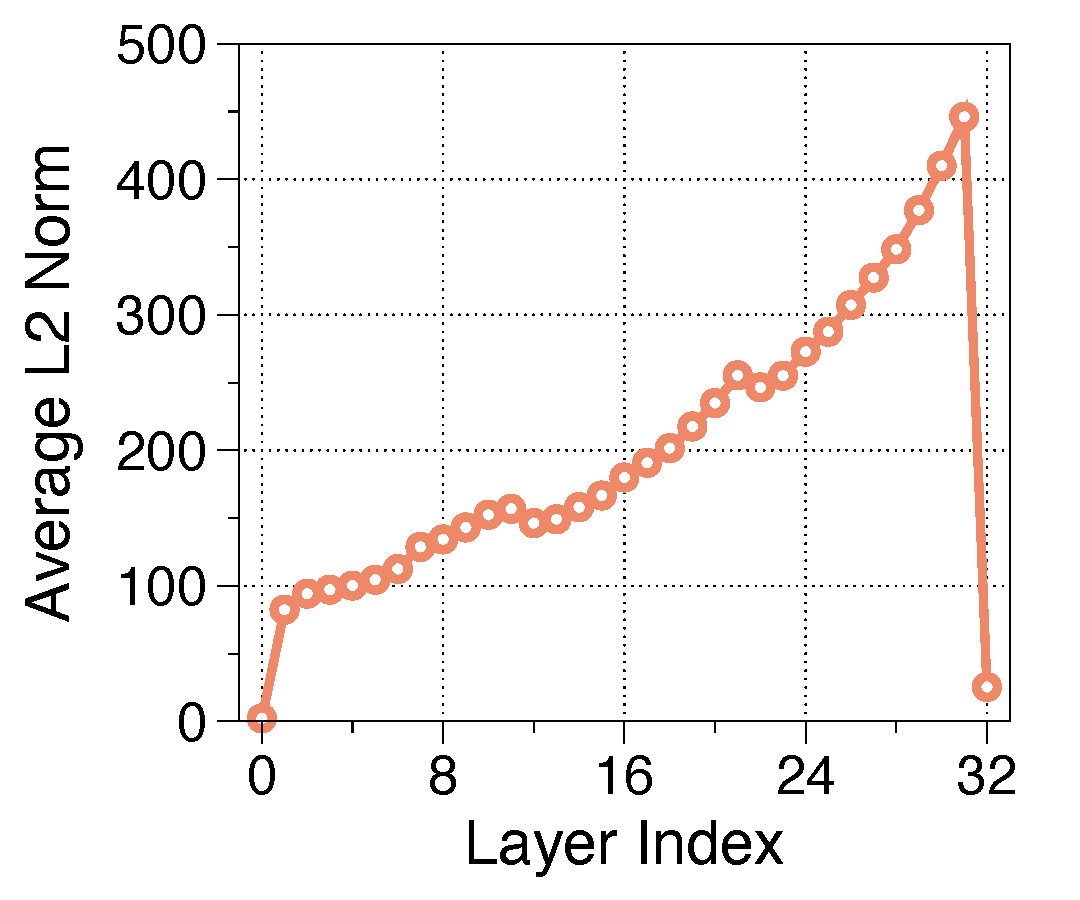
\includegraphics[width=\textwidth]{figs/kv_magnitude/mag_hidden.pdf}
        \subcaption{Hidden states}
    \end{subfigure}
    \centering
    \begin{subfigure}[t]{0.303\textwidth}
    \captionsetup{justification=centering}
        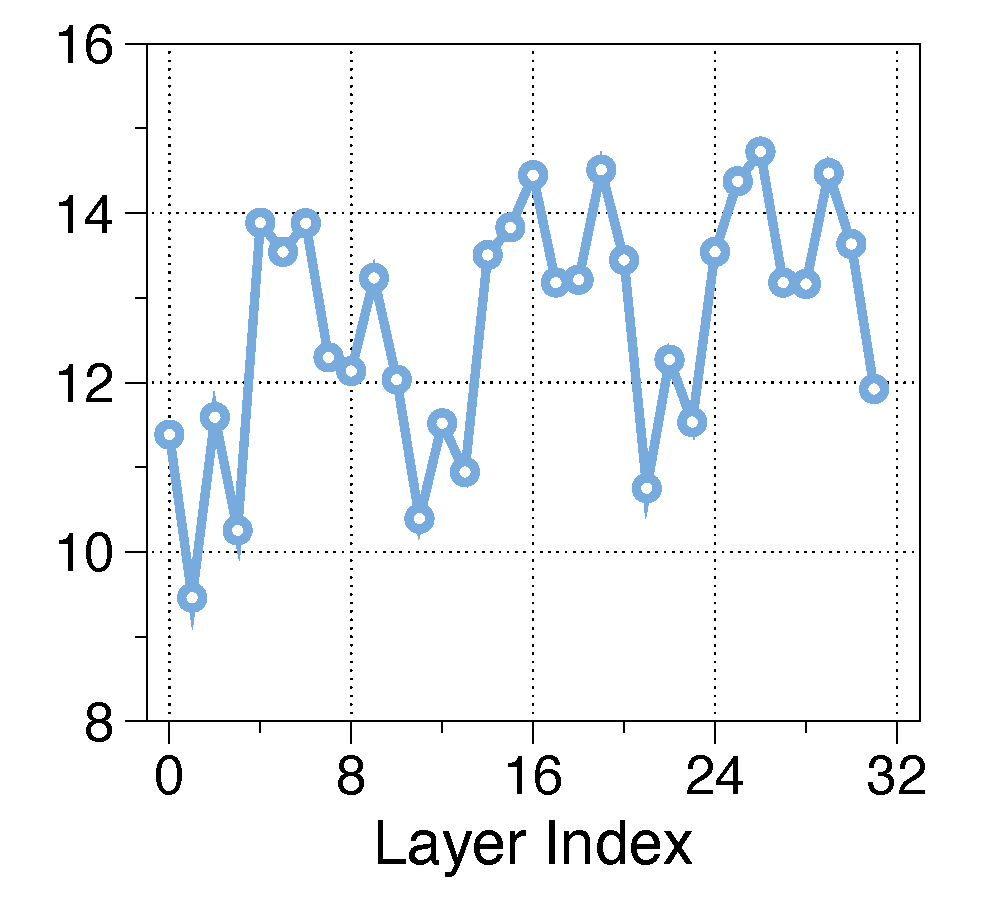
\includegraphics[width=\textwidth]{figs/kv_magnitude/mag_key.pdf}
        \subcaption{Key states}
    \end{subfigure}
    \centering
    \begin{subfigure}[t]{0.303\textwidth}
    \captionsetup{justification=centering}
        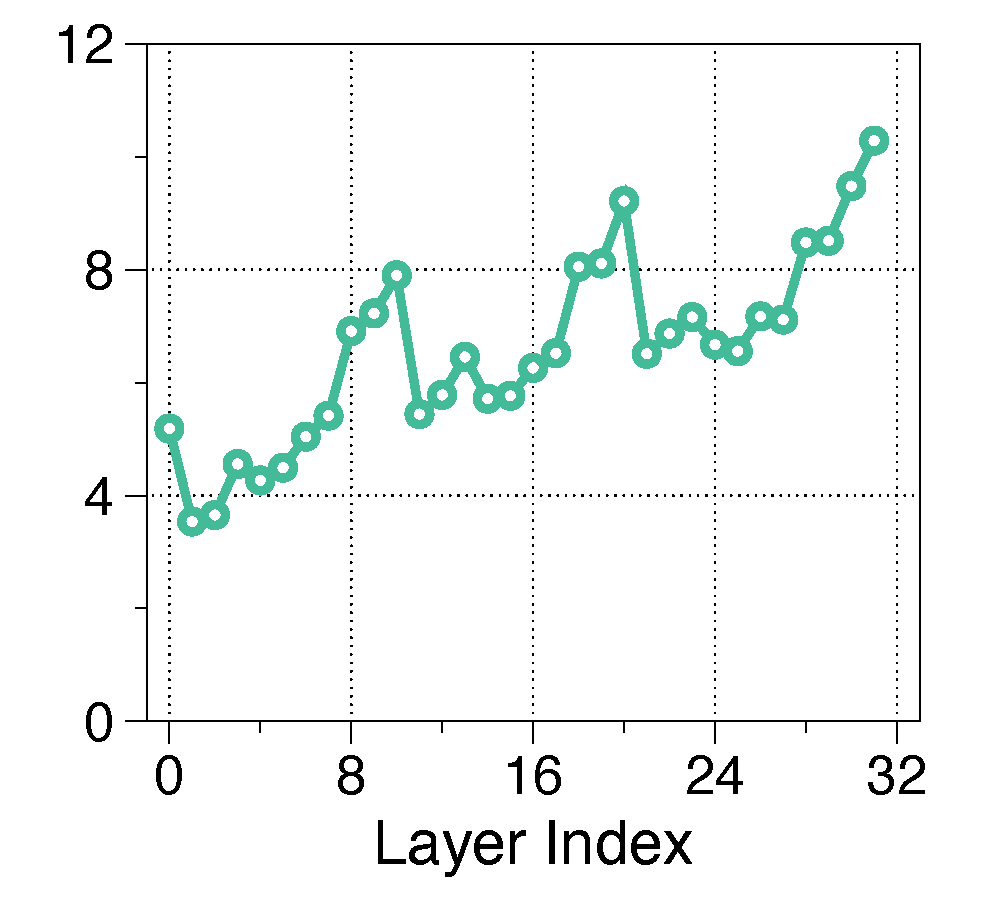
\includegraphics[width=\textwidth]{figs/kv_magnitude/mag_value.pdf}
        \subcaption{Value states}
    \end{subfigure}
    \caption{ Average L2 norm magnitude of (a) hidden states, (b) key states, and (c) value states across layers in a Middle-Cycled Recursive Transformer 360M with 3 recursion steps. 
    Note that the last hidden states correspond to the final hidden states after the last layer normalization. 
    }
    \label{fig:kv_sharing_mag_app}
\end{figure}